\chapter{Retningslinjer for bruk av rotårsaksanalyse innen informasjonssikkerhet}
\label{kap:retningslinjer-RCA}
Retningslinjene er skrevet slik at de kan bli benyttet uten bacheloroppgaven. Derfor vil noe av det som er gjennomgått i bacheloroppgaven bli gjentatt.

\section{Formål og bakgrunn}
Formålet med dette dokumentet er for å gi leseren en retningslinje på anvendelse av rotårsaksanalyse. Retningslinjen beskriver anvendelse av rotårsaksanalyseverktøyene beskrevet i boken ``Root Cause Analysis: Simplified Tools and Techniques - second edition'' av Bjørn Andersen og Tom Fagerhaug \cite{RCA}. Vi anbefaler denne boken som samlet metodikk. Boken beskriver godt hva som skal til for å komme frem til rotårsaken til et problem. 

Dette dokumentet ble skrevet i forbindelse med bacheloroppgave i informasjonssikkerhet der det ble gjennomført tre caser. Retningslinjene er derfor basert på funn fra disse casene, om hvordan metoden og verktøyene fungerte.

Dette dokumentet vil ikke beskrive vertkøyene, men valg av de. Beskrivelsen til verktøyene står i boken til Fagerhaug og Andersen \cite{RCA}.

\section{Valg av verktøy}
Boken beskriver 7 faser i rotårsaksanalyse. Disse må bli fulgt stegvis ettersom hver fase bygger på resultater fra foregående. Verktøyene beskrevet i boken til Fagerhaug og Andersen \cite{RCA} er generelle verktøy som er ofte brukt i rotårsaksanalyse. Vi har sett på et utvalg av disse verktøyene og hvordan disse fungerer innen informasjonssikkerhet. 

\begin{figure}[H]
    \centering
    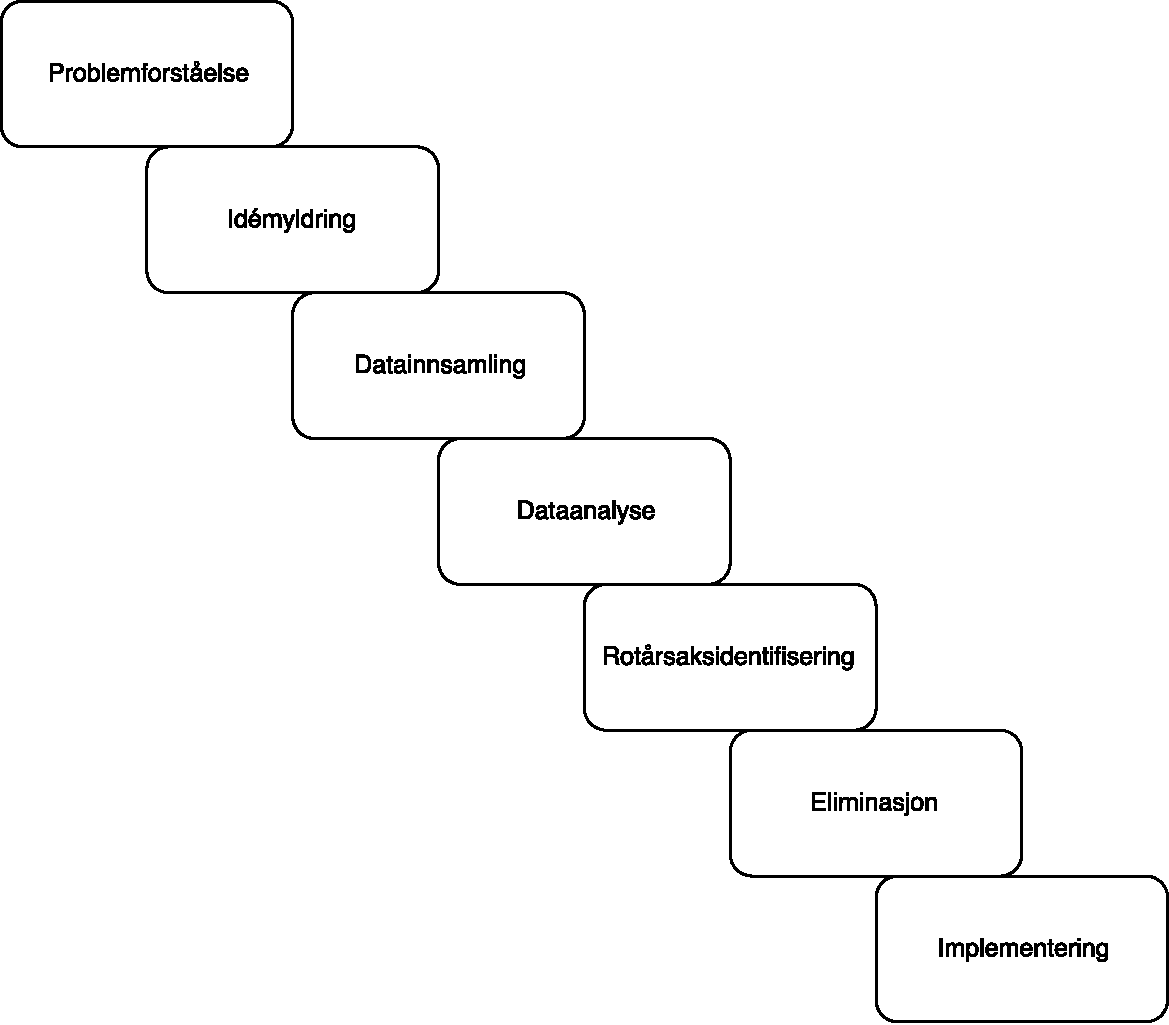
\includegraphics[scale=0.4]{prosess}
    \caption[RCA-prosess]{De syv fasene i rotårsaksanalyseprosessen}
    \label{fig:prosess}
\end{figure}
\subsection{Problemforståelse}
Problemforståelse går ut på å få en solid forståelse for problemet en ønsker å løse. Det kan også hjelpe med å skape enighet rundt hva problemet egentlig omfatter. Det er også viktig for å passe på at ressursene som benyttes for analysen brukes effektivt videre. 

Verktøyene vi anbefaler til denne fasen er: 
\begin{description}
    \item[Kritiske hendelser] Kritiske hendeleser er et godt verktøy å bruke når man har mye data, som kan gi et innblikk i hva som går galt. Innen IT pleier en å logge mye, noe som gir mye data.
\end{description}

\subsection{Idémyldring}
Målet med idémyldring er å generere så mange idéer som mulig om et gitt emne. I rotårsaksanalyse er målet stort sett å generere en liste over problemområder som kan forbedres, identifisere mulige konsekvenser, generere en liste over mulige årsaker til problemet og oppmuntre til å tenke på løsninger som kan eliminere problemet. 

Verktøyene vi anbefaler til denne fasen er:
\begin{description}
    \item[Idémyldring] Idémyldring gir mange idéer om mulige rotårsaker. Hvis det er noen som dominerende i gruppen som gjennomfører idémyldringen, burde idéskriving benyttes.
    \item[Nominell gruppe teknikk] Dette verktøyet gir en liste over hva en burde prioritere mest i datainnsamling for å gi ett godt datagrunnlag for å finne rotårsaken. Ved å bruke resultatene fra idémyldingen, får en prioritert disse idéene. 
\end{description}

\subsection{Datainnsamling}
Ustrukturert og tilfeldig problemløsning har en tendens til å bli svært unøyaktig. Strukturert rotårsaksanalyse gir derimot et godt grunnlag for blant annet datainnsamlingen, som er en av de sentrale fasene i prosessen.

\begin{description}
    \item[Sampling] Sampling er et godt verktøy for å begrense datainnsamling til de relevante gruppene. 
    \item[Spørreundersøkelser] Spørreundersøkelser er et godt verktøy for å få data fra de berørte personene. 
\end{description}

\subsection{Dataanalyse}
I denne fasen blir dataene analysert og visualisert. Hovedmålet er å avklare mulige rotårsaker som har innvirkning på problemet, og hvilke av de som har størst innflytelse. Under beskrives de ulike verktøyene som ble brukt for å analysere dataene.

Verktøyene vi anbefaler til denne fasen er:
\begin{description}
    \item[Histogram] Histogram fungerer veldig godt for å skape en visuell forståelse av dataene, som kan gjøre det lettere å se korrelasjoner mellom variabler. Det gir også en tilfredstillende fremstilling av dataen. 
    \item[Affinitetsdiagram] Affinitetsdiagram passer veldig godt med spørreundersøkelser, der det er kortsvar- eller langsvaroppgaver. Det gir mulighet for å gruppere svarene etter innhold i svarene. 
    \item[Statistisk analyse] Statistisk analyse er ikke i boken, men er noe analyse metode som fungerer veldig godt for å se korrelasjoner. Dette fungerer også ved å se på signifikansen.
\end{description}

\subsection{Rotårsaksidentifisering}
De foregående fasene skal ha generert en liste over mulige rotårsaker og målet i denne fasen er å identifisere de faktiske årsakene. Det kan kreve flere iterasjoner for å finne rotårsaken(e). 

Verktøyene vi anbefaler til denne fasen er:
\begin{description}
    \item[Årsak-virkning diagram] Som årsak-virkning anbefaler vi å benytte fiskebeindiagram. Ved å bruke fiskebeindiagram får en en visuell fremstilling av rotårsaken til problemet. 
    \item[5 Whys] Hvis det er mistanke om høyere årsaker bak de identifiserte årsakene kan 5 whys gi en bekreftelse på om årsakene identifisert er faktisk rotårsak og ikke lav-nivå årsaker. 
    \item[Feiltreanalyse] 
\end{description}

\subsection{Rotårsakseliminering}
Denne fasen innebærer å komme med mulige løsninger til problemet for å eliminere rotårsaken. Boken til Fagerhaug og Andersen \cite{RCA} beskriver to mulige tilnærminger til denne fasen. En tilnærming for å stimulere kreativitet når man leter etter løsninger, og en for å konstruere og utvikle løsninger.

Verktøyene vi anbefaler til denne fasen er:
\begin{description}
    \item[De seks tenkehatter]
    \item[SIT] 
\end{description}
Bruk SIT - så sant det ikke er fysiske krav. Da kanskje bruke TRIZ. 
Krever kreativ løsning, bruk 6 tenkehatter

\subsection{Løsningsimplementering}
I den siste fasen er målet å implementere løsningene som ble funnet i foregående fase. Implementeringen inkluderer blant annet organisering, utvikling av en implementeringsplan, skape et konsensus om de nødvendige endringene og selvfølgelig implementeringen. Implementeringen av løsningen kan sies å være en suksess når symptomene forsvinner. 

Verktøyene vi anbefaler til denne fasen er:
\begin{description}
    \item[Trediagram] Trediagram fungerer veldig bra for å lage en plan over hva som må gjøres for at tiltaket skal bli implementert. 
\end{description}
I dette steget er de ikke nødvendig å bruke noe verktøy, men det kan være lurt å benytte trediagram for å få en plan over løsningimplementering.

